% Made up for the tikra benchmark.
\usetikzlibrary{shapes.multipart, arrows.meta}
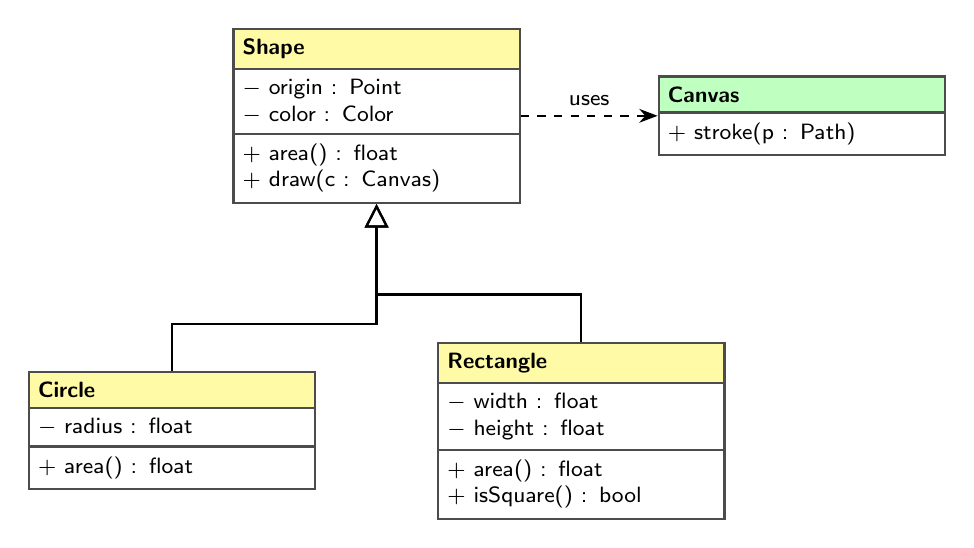
\begin{tikzpicture}[font=\sffamily\footnotesize,
    class/.style={rectangle split, rectangle split parts=3, draw=black!70, thick,
      rectangle split part fill={yellow!35, white, white}, text width=3.4cm, align=left},
    inherit/.style={-{Triangle[open, length=3mm, width=3mm]}, thick},
    assoc/.style={-{Stealth}, thick, dashed}]
  \node[class] (shape) at (0,0) {
    \textbf{\textit{Shape}}
    \nodepart{second} $-$ origin : Point\\ $-$ color : Color
    \nodepart{third} $+$ area() : float\\ $+$ draw(c : Canvas)};
  \node[class] (circle) at (-2.6,-4) {
    \textbf{Circle}
    \nodepart{second} $-$ radius : float
    \nodepart{third} $+$ area() : float};
  \node[class] (rect) at (2.6,-4) {
    \textbf{Rectangle}
    \nodepart{second} $-$ width : float\\ $-$ height : float
    \nodepart{third} $+$ area() : float\\ $+$ isSquare() : bool};
  \node[class, rectangle split parts=2, rectangle split part fill={green!25, white}] (canvas) at (5.4,0) {
    \textbf{Canvas}
    \nodepart{second} $+$ stroke(p : Path)};
  \draw[inherit] (circle.north) -- ++(0,0.6) -| (shape.south);
  \draw[inherit] (rect.north) -- ++(0,0.6) -| (shape.south);
  \draw[assoc] (shape.east) -- node[above] {uses} (canvas.west |- shape.east);
\end{tikzpicture}
